\documentclass [a4paper, 12pt]{article}

\usepackage{amssymb}
\usepackage{epsfig}
\usepackage{graphicx}
\usepackage{times}
\usepackage{float}
\usepackage[usenames,dvipsnames]{color}
\usepackage{pgfplotstable}
\usepackage{pgfplots}
\usepackage{natbib}
 \usepackage{tikz} 
\usepackage{xspace}

\usepackage[colorinlistoftodos,prependcaption,textsize=tiny]{todonotes}

\newcommand{\unsure}[2][1=]{\todo[linecolor=red,backgroundcolor=red!25,bordercolor=red]{#2}}
\newcommand{\change}[2][1=]{\todo[linecolor=blue,backgroundcolor=blue!25,bordercolor=blue]{#2}}
\newcommand{\info}[2][1=]{\todo[linecolor=OliveGreen,backgroundcolor=OliveGreen!25,bordercolor=OliveGreen]{#2}}
\newcommand{\improvement}[2][1=]{\todo[linecolor=Plum,backgroundcolor=Plum!25,bordercolor=Plum]{#2}}

\newcommand{\julich}{J\"ulich\xspace}

\textwidth 16 cm
\textheight 23 cm
\setlength{\oddsidemargin}{0.1 cm}
\setlength{\topmargin}{1 cm}
\setlength{\headheight}{0cm}
\setlength{\headsep}{0cm}
\setlength{\footskip}{0.75cm}
\setlength{\parindent}{0cm}
\setlength{\oddsidemargin}{0.1 cm}
\setlength{\itemsep}{10pt}

 
\begin{document}

\begin{center}
{\LARGE \bf Project Proposal for HPC Access to JURECA and JUWEL} 

\bigskip
\bigskip
\bigskip
\end{center}
\textbf{Period}
\phantom{MM}\textit{01.05.2018 - 30.04.2019 }

\bigskip
\textbf{Project title}\\
\phantom{MM}\textit{Arbor Big Scaling}

\bigskip
\textbf{Type of project}\\
\phantom{MM} \textit{New project}

\bigskip
\textbf{Principal investigator}\\
\phantom{MM} \textit{Dr. Alexander Peyser, Forschungszentrum \julich }

\bigskip
\textbf{Project contributor(s)}\\

\begin{itemize}
\item \phantom{MM} \textit{Wouter Klijn, Forschungszentrum \julich }
\item \phantom{MM} \textit{Ben Cumming, Swiss National Supercomputing Center, Switzerland}
\item \phantom{MM} \textit{Stuart Yates, Swiss National Supercomputing Center Switzerland}
\end{itemize}

\newpage

\vfill
\tableofcontents
\vfill

\newpage



\section{Introduction}
\rule{\textwidth}{0.4pt}\\

\textit{Give a short outline of the scientific background of your research, including references.}\\
Current and future HPC systems are increasingly include heterogenious many-core architectures like GPUs and Knights landing. Arbor is a new morphologically detailed neural simulator designed to exploit these architectures . Designing  from the ground-up for heterogeneous and many-core systems it aims to exploid the potential of these large systems for the neuroscientific community. 

The performance of Arbor has been tested on small HPC resources and good scaling has been shown on medium to large systems. These tests where done with very constraint and simplistic network. In this compute time proposal we ask time to perform scaling experiments on the diverse compute resources available in \julich with two neural networks having both a realistic spike rate and biologically realistic connectivity pattern. This will allow us to assertain the performance under realistic loads.

The models used for benchmarking are a simplified cortical model based on 1,2 and a hippocampus model based on 3,4. In pilot experiments it was established that with under specific parameter settings these networks have a property essential for scaling experiments: The networks can be scaled up to arbitrary size without 

\textit{(about 1 page)}
\section{Preliminary Work}
\rule{\textwidth}{0.4pt}\\
\textit{Provide a brief summary of your preliminary work in connection with the proposed project, including references.}\\

The Arbor simulator has not yet had an official release. Development is done in an open fassion, the software has been online available online for more then a year (5). Preliminiairy results have been presented at numerous accacions in the form of posters and presentation.


Dry run mode

Big scaling week

pilot experiments


\textit{(about 1 to 2 pages)}
\section{Description of the Project}
\rule{\textwidth}{0.4pt}\\
\subsection{Project Details}
%\textit{Describe your research project in detail, structured in sub-projects, if applicable. Include discussion of the scientific questions that you are planning to address and the overall scientific goals of the project. It is important that you describe the innovative aspects, impact and topicality of the proposal.}

im of the project is to validate the large scale performance of the Arbor simulator on large systems, while simulating two models with biological realistic spike rate and bulk connectivity. 
Two biological systems at extremes of these two 

\begin{itemize}\setlength{\itemsep}{-2pt}
  \item Scientific questions you want to address
Validation of the performance of the spike communication under realistic load. For a diverse set of realist models with divert levels of details in the cel simulations. 
  \item Scientific objectives
This compute time proposal only has computational aspects. No specific scientific questions will be explored.

  \item Computational objectives
A number of different internode and intra node exchange methods have been implemented for Arbor. What method is optimal for the different hardware architectures and loads is currently not known. A dryrun mode is available for initial estimations of performance, This method can not reproduce the exact resource load. Cache cehorence and memory bandwith bottlenecks are highly depending on the workload and different hardware configurations available.

 \item Approach and expected outcome
The different communication methods currently available will be compared for a predetermined set neuroscientific models. Each models with increasing complexity and shifting workloads. If major bottle necks are encountered these will be investigated and hopefully alleviated.

  \item Expected impact on the research area
The Arbor simulator will allow large scale simulations of morphologically detailed neural networks on many-core architectures. Like the knight landing, GPU's and at a later stage FPGA and the Chinese hardware (ref)

  \item Scientific and technical innovation potential
The Arbor software is developed with a modular approach: The different components are abstracted with clear internal APIs this allows other simulators to reuse components to improve performance or expand  capability. 

  \item Progress beyond the state-of-the-art

\end{itemize}

\subsubsection{Sub-project 1}

\subsubsection{Sub-project 2}

\textit{(1 to 2 pages per sub-project)}
\subsection{Review Processes}
\textit{Has the underlying research project already successfully undergone a scientific review process? Is the project funded by public money?
If yes, please also provide information about the funding source
(e.g. State, BMWi, BMBF, DFG, EU, $\dots$)}
\section{Numerical Methods and Algorithms} 
\rule{\textwidth}{0.4pt}\\
\textit{Describe the numerical methods and algorithms that you are planning to use, improve, or develop.}\\
 
\textit{(1 to 2 pages)}
\bigskip

\section{Computer Resources}
\rule{\textwidth}{0.4pt}\\
\subsection{Code performance and workflow}
\textit{Describe the codes, packages or libraries that you need to undertake the project, and how these will enable the research to be achieved. Include for \textbf{each code to be used} information about}
\begin{itshape}
\begin{itemize}\setlength{\itemsep}{-2pt}
  \item Which code will be used
The code used can be found at (6). 

  \item How is the code parallelized (pure MPI, mixed MPI/OpenMP, Pthreads, CUDA, etc.)
The Arbor simulator is build with multiple backends in mind. The paralllization is thus diverse. The node paralellizetion is performed with MPI. Node threading is performed with the Intel Tread  building blocks and a hardwritten C threads librairy. Further paralellizetion is done depending on the many-core backend: vectorization with AVX on the appropriate backend including intrinsics. For GPUs Cuda is used.

  \item The amount of memory necessary (per core, per node and in total)
The amount of memory used is minimal. Running a network with 400000 neurons, ten times more then typically expected, uses a maximum of 1712.982 MB on a KNL system. Arbor is compute limitted in the extreme and memory constraints are not under considiration.

  \item Scaling plots \textbf{and} tables with speedup results for runs with typical, parameter sets, problem size, and I/O \textbf{of the planned project} (no general benchmark results are accepted)
  \item Describe architecture, machine/system name, and problem size used for the scaling plots
  \item Current job profile (independent jobs, chained jobs, workflow, etc.)
\end{itemize}
\end{itshape}

{\it \textbf{Important:} please take into account the corresponding technical guidelines and requirements (e.g. required minimal code scalability, memory restictions, etc.) of the machine you have chosen!}\\
 \cite{NEST_2_12}.

\begin{table}[H]
	\caption{\label{tab_scaling} Scaling behavior}
	\begin{center} 
	\setlength{\tabcolsep}{10pt}
		\renewcommand{\arraystretch}{1.2}
		\begin{tabular}{lrr}
			\#cores  & absolute timing (s) & speedup\\ \hline
			3	 & 600        &    1.0  \\ 
			6        & 600       &    2.0   \\
			24        & 600        &    8.0   \\
			48       & 600        &   16.0   \\
			96       & 600        &   32.0   \\
			192       & 600         &   64.0   \\
			384      & 600         &  128.0   \\
			768      & 600         &  256.0   \\
			1536      & 600         &  512.0   \\
			3000     & 600          &  1000.0   \\
			
		\end{tabular}
	\end{center}
\end{table}

\begin{figure}[H]
\begin{tikzpicture}
\begin{axis}[
  xlabel=Cores,
  ylabel=Simulation time in s,
  xmin=0, xmax=3000,
  ymin=0, ymax=6000,
  title={Weak scaling for increasing number of network instances}]
\addplot [color=blue, mark=square,]
coordinates {
    (3,600.0)(6,600.0)(12,600.0)(24,600.0)(48,600.0)(96,600.0)(192,600.0)(384,600.0)(768,600.0)(1536,600.0)(3000,600.0) 
    };
    \addlegendentry{Simulation times}
]
\end{axis}
\end{tikzpicture}
\caption{Weak scaling for increasing number of network instances with different parameters on increasing number of cores. Each instance of the network is independent from each other, thus having a perfect linear scaling.}
\end{figure}


\newpage
\subsection{Justification of resources requested}
\setlength{\tabcolsep}{4pt}
\begin{tabular}{l|c|c|c|c|c}
   Sub-project & Size (neurons) & nodes /run JuropaTest    & core-h /run & \# runs  & core-h \\ \hline

  \textbf{Sub-project 1}  &               &                &             &          &              \\
  100 neuron network      	  & $1\cdot 10^2$ & 125 (3000 cores)    & 3000*5=15000    &  300 & 4,500,000      \\
  
  
\end{tabular}
\bigskip

\noindent Total requested time on JURECA: {\tt } 4,500,000 core-h\\
\noindent 125 cores/run will be used.\\


\section{Resource Management and Work Schedule}
\rule{\textwidth}{0.4pt}\\
\subsection{Resource management}
\textit{Describe how you intend to manage the resources you have requested. This should include a description of the methods you will deploy to monitor progress of the project and how project results are documented.}\\

\textit{(0.5 to 1 page)}

\subsection{Work schedule}

\bigskip
\textit{Gantt chart for the project Learning to Learn}
\begin{figure}[H]
\begin{flushleft}
 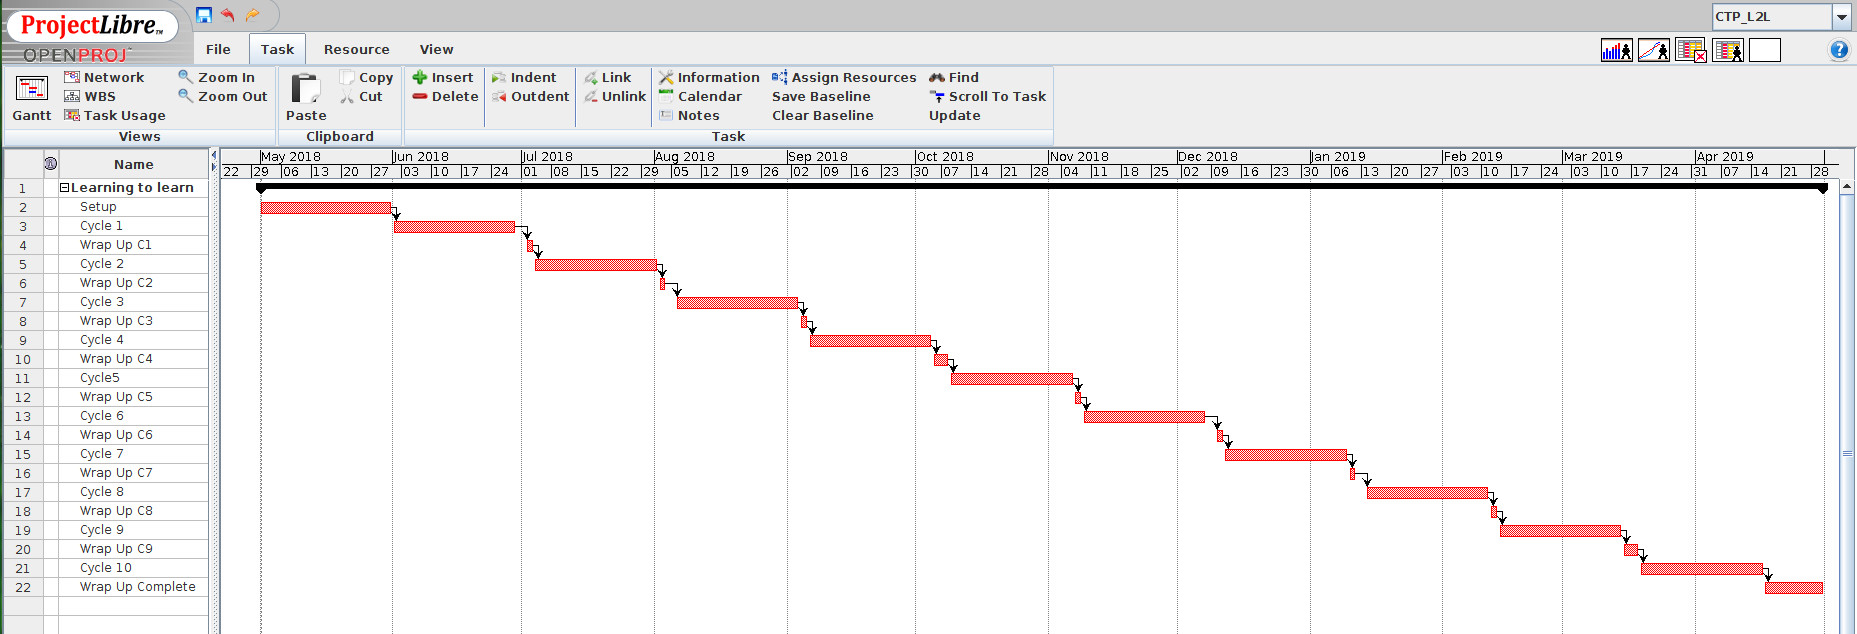
\includegraphics[scale=0.25]{Figures/gantt_chart.jpg}
\end{flushleft}
 \caption{\label{fig_workschedule}Work schedule for the project.}
\end{figure}

\section{Key Personnel and Experiences}
\rule{\textwidth}{0.4pt}\\
\textit{Give a short introduction of the key persons involved in the project and their experience (max 3 persons).}\\

\textit{(half a page)}
\newpage

\section{Bibliographic References}
\rule{\textwidth}{0.4pt}\\
\bibliographystyle{plain}
\bibliography{references}

\bigskip
\begin{flushright}
{\tiny V1.4-2017JUL05}
\end{flushright}
\end{document}
